% !TEX root = Master.tex

The same procedure as in Subsection \ref{sssec:margin_kcc_6} for key category cluster 2 will be applied here to analyze the marginal distribution of the log-sales in key category cluster 6.\\

Excluding all covariates, simple maximum likelihood estimation results can be summarized within \autoref{tab:estimated_parameters_kcc_6_no_covariates}, \autoref{fig:kcc_6_marginal} and \autoref{fig:res_kcc_6_no_covariates}. A Shapiro-Wilk test on the residuals returns a p-value of 0.87 and the fails to reject the null hypothesis of non-normality.
\\



\begin{table}[H]
\setlength\arrayrulewidth{1pt}  
\centering
\begin{adjustbox}{max width=\textwidth}\
\begin{tabular}{|c|c|c|}
\hline
\rowcolor{lightgray} 
$\hat{\mu}$ & $\hat{\sigma}$ & $\hat{\nu}$ \\ \hline
9.62        & 0.20           & 0.41        \\ \hline
\end{tabular}
\end{adjustbox}
\caption{Estimated parameters for log-sales of KCC 6 fitted to exGaussian distribution with no covariate effects}
\label{tab:estimated_parameters_kcc_6_no_covariates}
\end{table}



 \begin{figure}[H]
\centering
\begin{subfigure}{.45\textwidth}
  \centering
  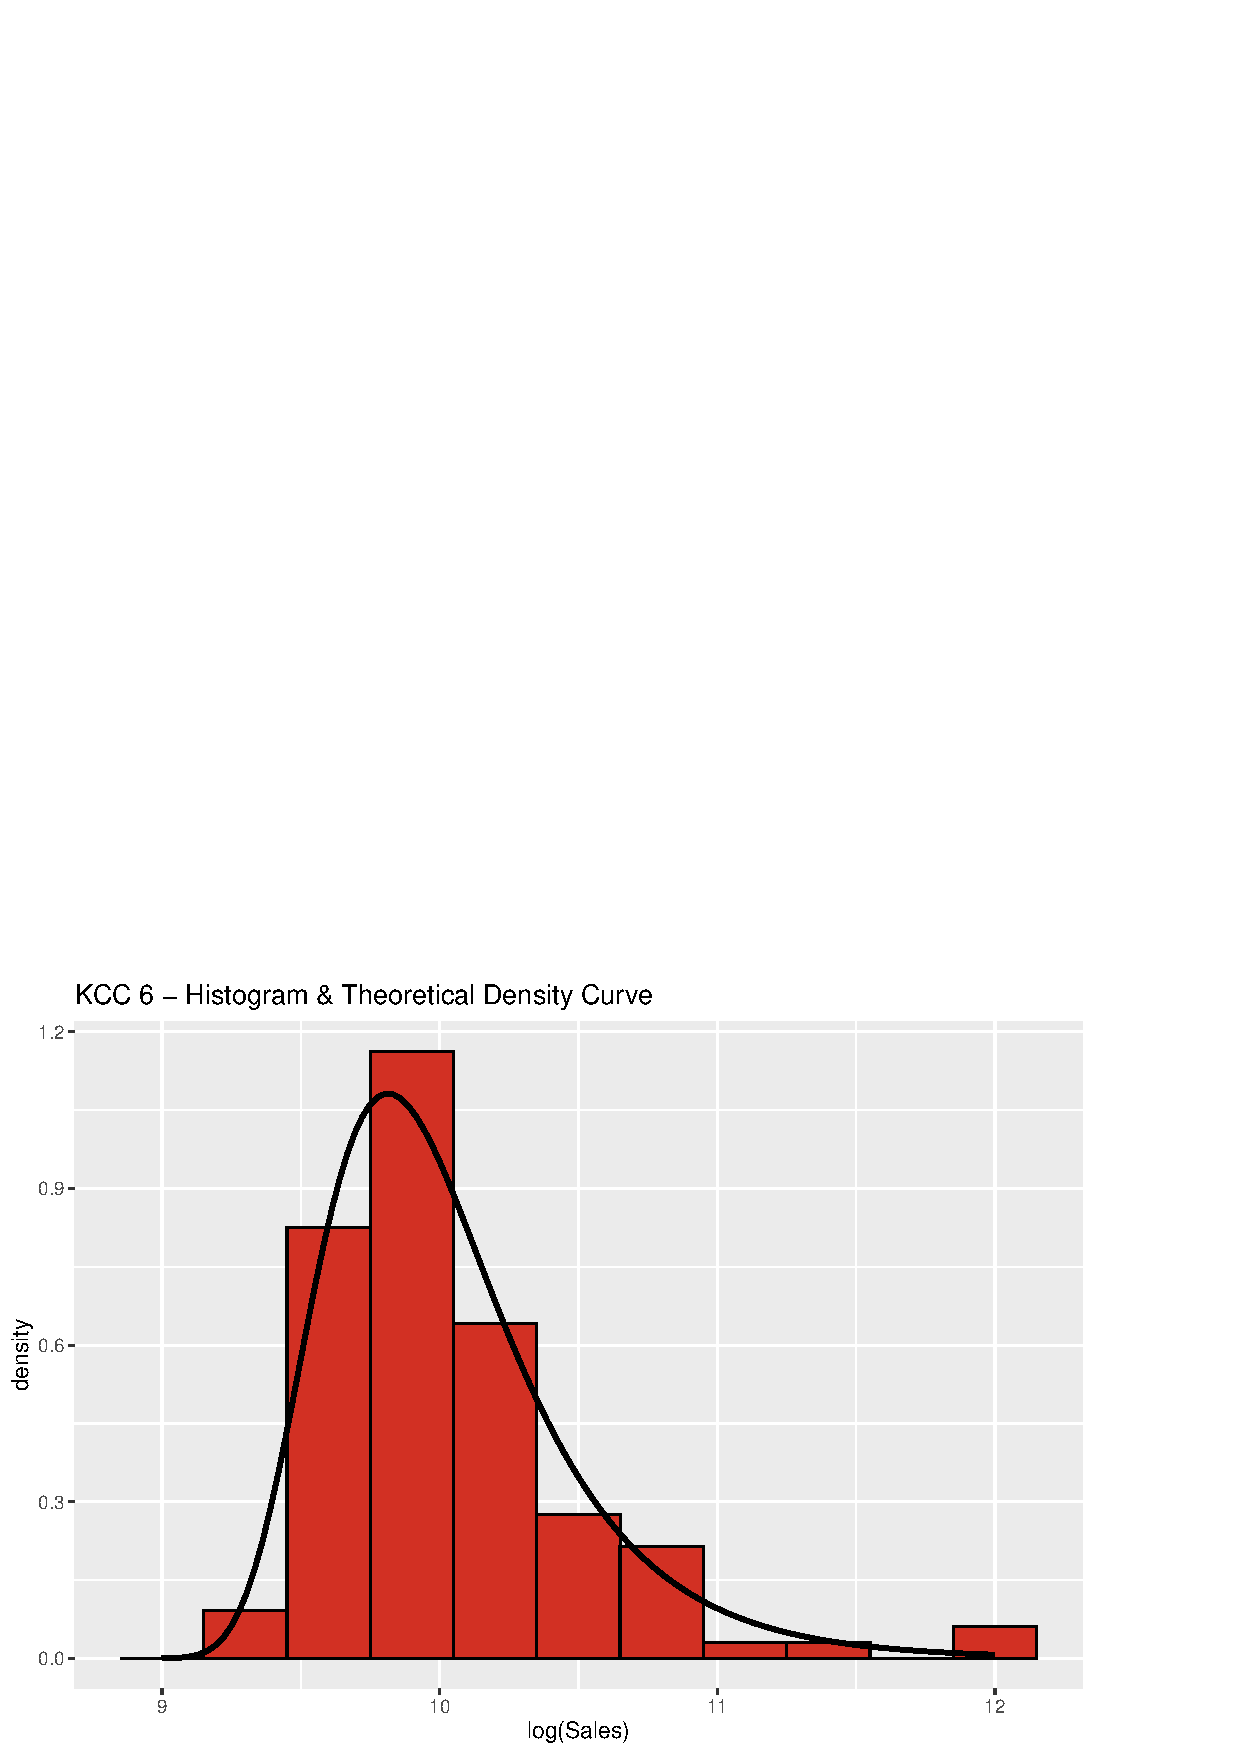
\includegraphics[width=\linewidth]{figures/kcc_6_density.png}
  \caption{Histogram \& theoretical density}
  \label{fig:kcc_6_density}
\end{subfigure}
\begin{subfigure}{.45\textwidth}
  \centering
  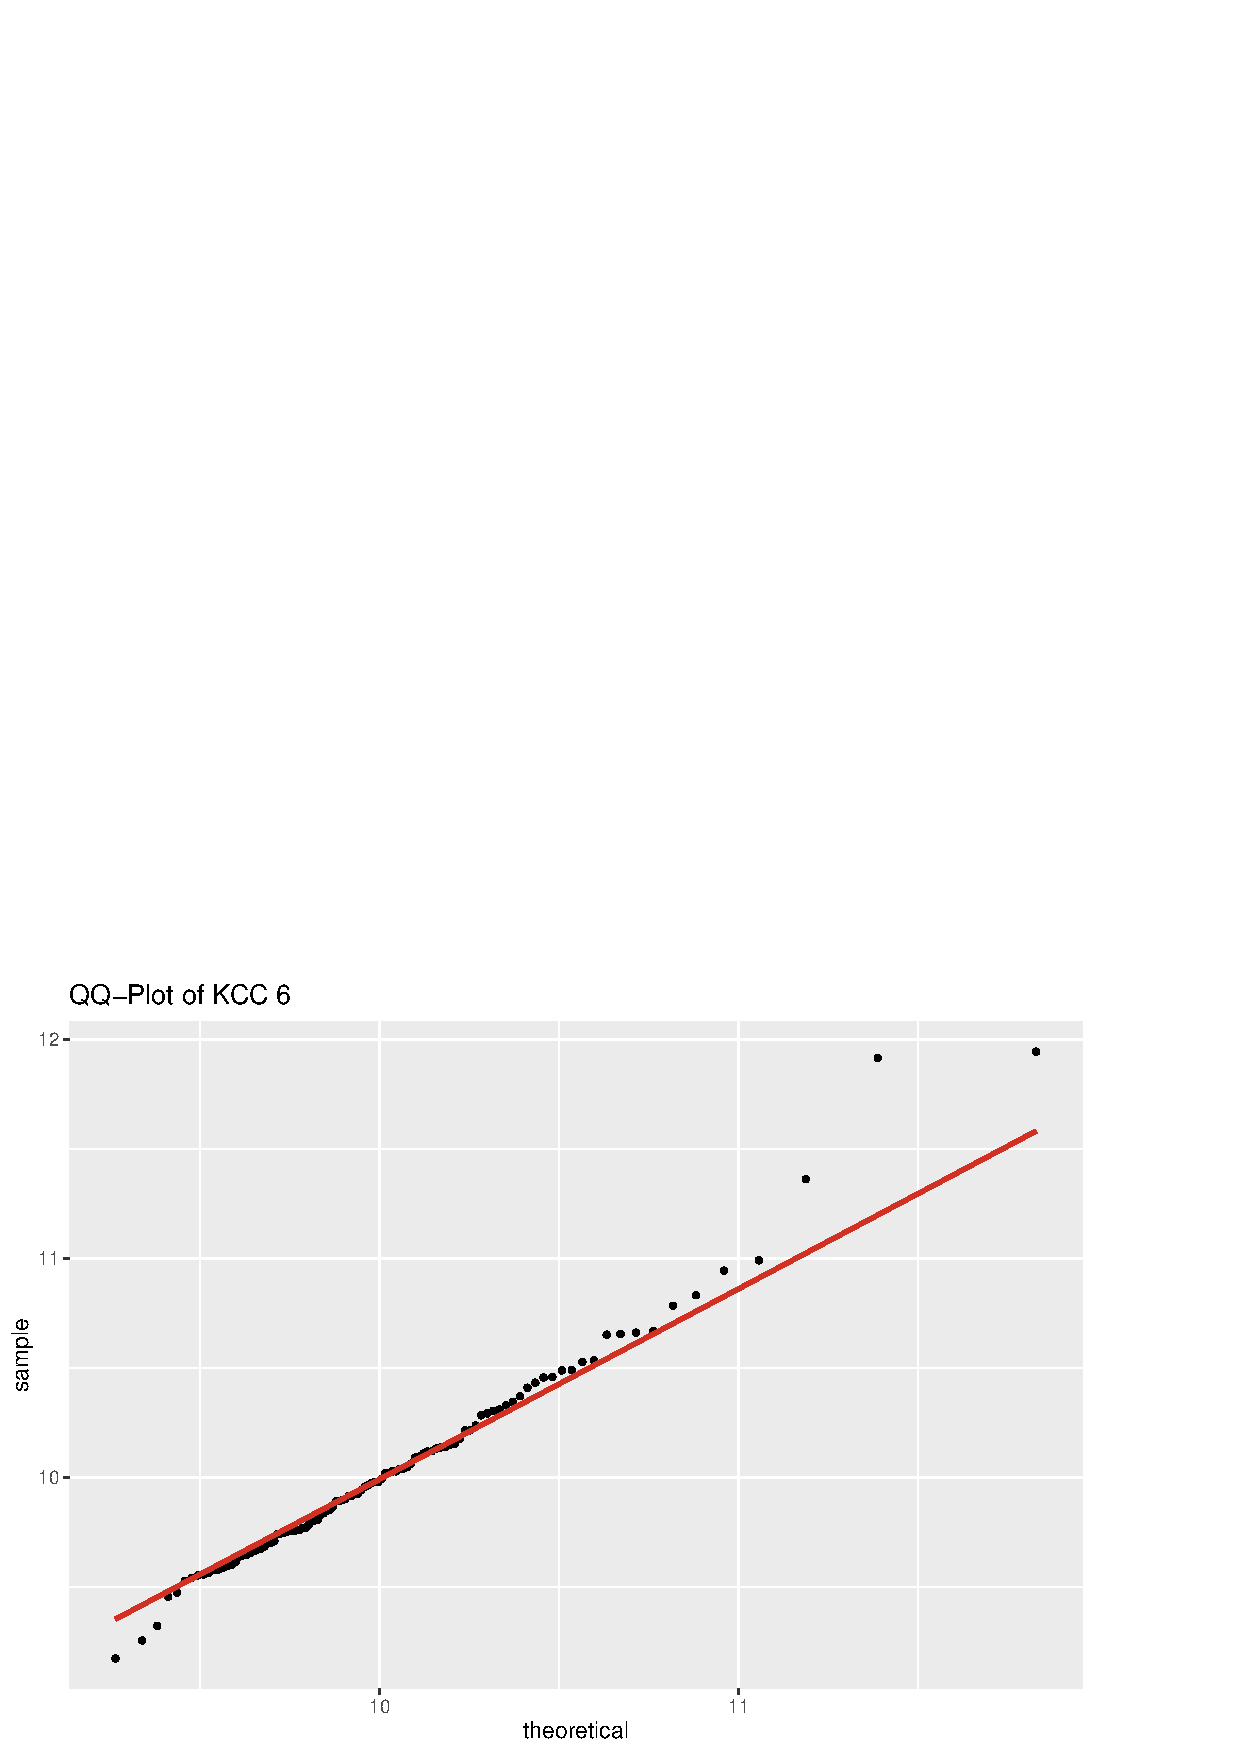
\includegraphics[width=\linewidth]{figures/kcc_6_qqplot.png}
  \caption{QQ-Plot}
  \label{fig:kcc_6_qqplot}
\end{subfigure}
\caption{exGaussian distribution fitted to log-sales of \ac{KCC} 6}
\label{fig:kcc_6_marginal}
\end{figure} 


\begin{figure}[H]
\centering
  \includegraphics[width=0.45\linewidth]{figures/res_kcc_6_no_covariates.png}
  \caption{Residuals of KCC 6 log-sales fitted to an exGaussian distribution with no covariate effects together with their density curve}
  \label{fig:res_kcc_6_no_covariates}
\end{figure}


Reviewing different model specifications, the same issues as for \ac{KCC} 2 arise when including Black Friday and Friends \& Family promo activations. Therefore, the same models as in the previous Subsection is chosen (Model \ref{eq:gamlss_kcc_2}, exGaussian distribution family for the response variable). 
%A summary output is printed below.
The estimated time-varying location and scale parameters can be seen in \autoref{fig:gamlss_kcc_6_estimated_parameters} and the skewness parameter $\hat{\nu}$ with 95\% CI in \autoref{tab:nu_ci_kcc_6}. The standard deviation remains almost constant at 0.2, uncertainty taken into consideration.
\\


\VerbatimInput[frame = single, label = "GAMLSS Fit on KCC 6" ]{gamlss_fit_kcc_6_try1.txt}



\begin{figure}[H]
\centering
  \includegraphics[width=0.95\linewidth]{figures/gamlss_kcc_6_estimated_parameters.png}
  \caption{Estimated location parameter $\hat{\mu}$ and scale parameter $\hat{\sigma}$ with confidence bands of GAMLSS fit - KCC 6}
  \label{fig:gamlss_kcc_6_estimated_parameters}
\end{figure}



\begin{table}[H]
\setlength\arrayrulewidth{1pt}  
\centering
\begin{adjustbox}{max width=\textwidth}\
\begin{tabular}{|c|c|c|}
\hline
\rowcolor{lightgray} 
Lower & $\hat{\nu}$ & Upper \\ \hline
0.040        & 0.021           & 0.060        \\ \hline
\end{tabular}
\end{adjustbox}
\caption{Estimated skewness parameter $\hat{\nu}$ of GAMLSS fit with 95\% confidence interval bounds - KCC 6}
\label{tab:nu_ci_kcc_6}
\end{table}



\autoref{fig:gamlss_effects_kcc_6} reveals some interesting points regarding covariate effects. The temporal effect, just like the total markdown percentage, collapses to an increasing straight line. The temporal effect also exhibits symmetrical behaviour around zero, including uncertainty. Just like in \ac{KCC} 2, the effect of Spring-Summer is slightly smaller than that of Fall-Winter.
\\






\begin{figure}[H]
\centering
  \includegraphics[width=0.95\linewidth]{figures/gamlss_effects_kcc_6.png}
  \caption{Covariate effects on the expected response variable (log-sales) of GAMLSS fit - KCC 6}
  \label{fig:gamlss_effects_kcc_6}
\end{figure}




Inspecting the diagnostic plots for the residuals in \autoref{fig:gamlss_residuals_kcc_6} along with the associated summary output, we can again confirm an appropriate fit.
\\



\begin{figure}[H]
\centering
  \includegraphics[width=0.95\linewidth]{figures/gamlss_residuals_kcc_6.png}
  \caption{Residuals of GAMLSS fit - KCC 6}
  \label{fig:gamlss_residuals_kcc_6}
\end{figure}


\VerbatimInput[frame = single, label = "Residuals of GAMLSS Fit on KCC 6" ]{gamlss_residuals_kcc_6.txt}
















